\subsection{Messung B}

Im folgenden Abschnitt soll die Probe B analysiert und die elektrosche Quadropolaufspaltung im Kern gezeigt werden.
Dazu wird der elektrische Feldgradient in $z$- Achse berechnet.
Der Aufbau des Versuchs ist mit dem aus Messung \ref{TODO:linkToAufbau} gleich, lediglich die Probe wurde ausgetauscht.
Der Auswertung in diesem Abschnitt liegt die in Abb. \ref{fig:velocityB} zu sehende Kalibrierung zu Grunde.
Diese Kalibrierungsmessung basiert auf der in Abschnitt \ref{TODO:linkToJannik} beschriebenen Methodik.

\begin{figure}[ht]
	\centering
	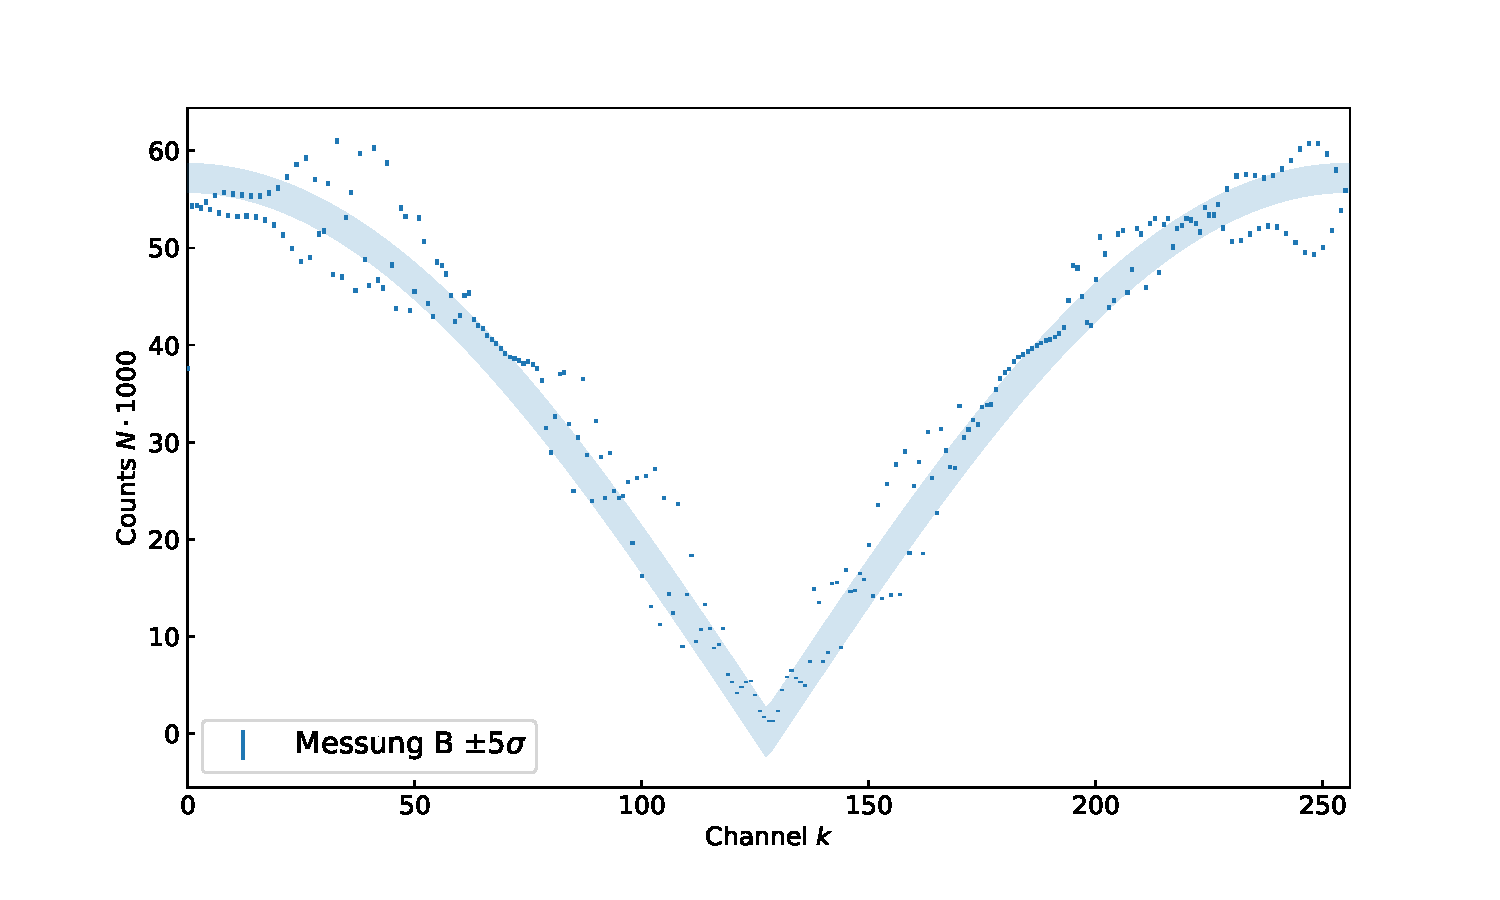
\includegraphics[width=0.7\textwidth]{dat/velocityB.pdf}
	\caption{Kalibrierung für die Messung B. Eingezeichnet sind die ungefilterten Messwerte und die Fitfunktion mit $A = (5,721 \pm 0,030) \cdot 10^4$ und $\Phi=0,4 \pm 0,7$.}
	\label{fig:velocityB}
\end{figure}

Die Amplitude dieser Kalibrierungsmessung liegt deutlich über deren der anderen Messungen.
Dies könnte an einer geringeren Masse der Probe B liegen.

\\

Nach einer Fehlmessung musste die Messung B nachträglich inklusive Kalibrierung widerholt werden.

\subsubsection{Isomerieverschiebung}

Um die Isomerieverschiebung zu erhalten, wird das Spektrum der durch den Absorber transmittierten Strahlung aufgenommen.
Das Signal wird mit einem Diskriminator auf den zu untersuchenden Bereich um $\SI{14,4}{\kilo\electronvolt}$ beschränkt
	und über einen Analog-Digital-Wandler auf den Computer gebracht.
Das gemessene Spektrum ist in Abb. \ref{fig:IsomerieB} zu sehen.
Bei dieser zweiten Messung des Spektrums wurde die Intensität über 40000 Iterationen addiert, um eine größere Statistik zu erhalten.

\begin{figure}[ht]
	\centering	
	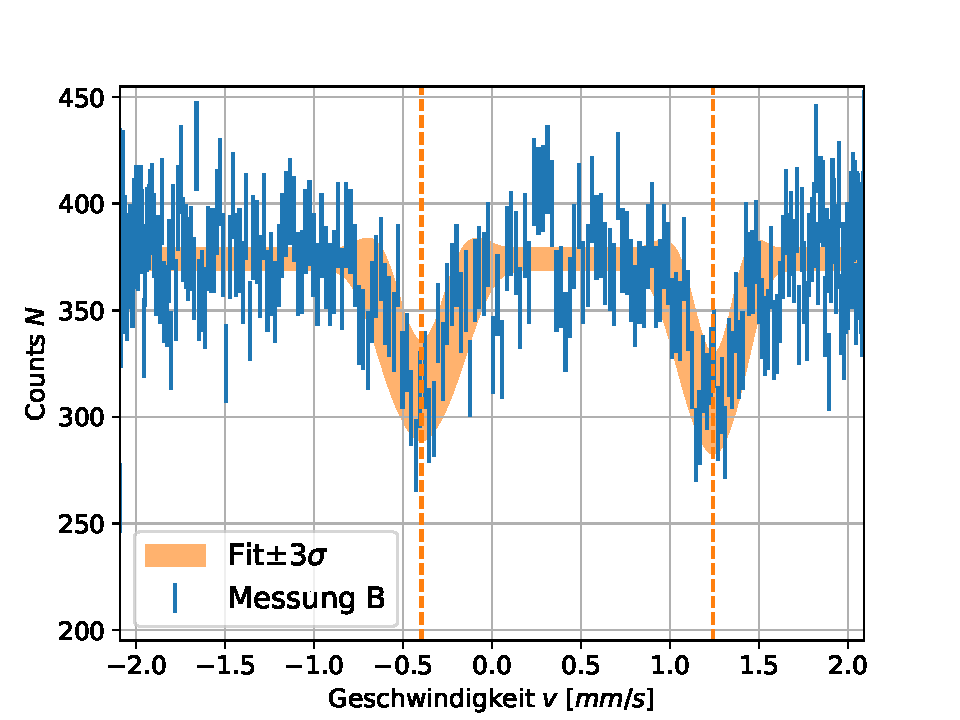
\includegraphics[width=0.8\textwidth]{dat/messungB.pdf}	
	\caption{Isomeriemessungen für Probe B.
		Es ist ein Gaußfit mit zwei Peaks eingezeichnet.
		Die Positionen der Peaks sind der Tab. \ref{isoB} zu entnehmen.
		Aus dem Mittel beider Peaks ergibt sich $v_\test{iso, B} = \input{dat/messungB_iso.txt}$.}
	\label{fig:IsomerieB}
\end{figure}

Da die Aufspaltung durch elektrische Quadropolwechselwirkung gleichmäßig ist, kann hier die Isomerieverschiebung durch Mittelung beider Peakpositionen auf
\begin{equation*}
	v_\text{iso, B} = \frac{v_1 + v_2}{2} = \input{dat/messungB_iso.txt}
\end{equation*}
ermittelt werden.
Damit lässt sich das Material des Absorbers auf $Na_2Fe(CN)_5NO \cdot 2H_2O$ bestimmen, welches laut \ref{TODO:Materialvergleich} eine Isomerieverschiebung
	relativ zu $^{57}$Fe in Pd von \Si{-0.4374 \pm 0.0018}{\milli\meter\per\second} aufweist.

Die entsprechenden Aufspaltungsenergien beider Zustände können in Tab. \ref{tab:isoB} abgelesen werden.
Sie ist definiert als Differenz von Anregungsenergie zu Isomerieverschiebung.

\begin{table}[ht]
	\centering
	\caption{Energieaufspaltungen beider Peaks von Probe B.} 
	\label{tab:isoB}
	\begin{tabular}{c|ccc}
		\toprule
		       &       $v_\text{res}$         &     \Delta v_\text{iso}      &     $\Delta E_\text{iso}$     \\ \midrule
		Peak 1 & \input{dat/messungB_x_1.txt} & \input{dat/messungB_v_1.txt} & \input{dat/messungB_E_1.txt}  \\
		Peak 2 & \input{dat/messungB_x_2.txt} & \input{dat/messungB_v_0.txt} & \input{dat/messungB_E_0.txt}  \\ \bottomrule
	\end{tabular}
\end{table}

\subsubsection{Elektronendichte}

Um die Elektronendichte $\abs{\Psi(0)}^2_\text{A}$ des Absorbers im Kern zu ermitteln, wird Gl. \ref{TODO:formelElektronendichteInAnleitung} nach

\begin{equation}
\abs{\Psi(0)}^2_\text{A} = \frac{5 v_\text{iso} E_\gamma \varepsilon_0}{S'(Z = 26) c e^2 Z R^2} \frac{1}{\frac{\Delta R}{R}} + \abs{\Psi(0)}^2_\text{Q} = \input{electrondensity_B.txt}
\end{equation}

\noindent umgestellt.
Dabei ist $\frac{\Delta R}{R} = TODO:value(dRR)$ aus \ref{TODO:jannikTeilAdRR} bekannt und die Elektronendichte $\abs{\Psi(0)}^2_\text{Q} = \SI{11881,8}{a_0^{-3}}$ von $^57$Fe in Pd gegeben.
Weiter sind $E_\gamma = \SI{14,4}{keV}$ die Quellphotonenenergie, $Z=26$ die Ordnungszahl von Eisen,
    $S'(Z = 26) = 1,33$ der relativistische Korrekturfaktor von Eisen und $R = 1,3 \cdot A^\frac{1}{3} \SI{\femto\meter}$ der Kernradius mit $A=57$ für Eisen.

\subsubsection{elektrischer Feldstärkegradient}

Da die Aufspaltung  in Fig. \ref{fig:IsomerieB} auf ein elektrisches Quadropolmoment zurückzuführen ist,
	kann mit der Aufspaltungsenergie der Gradient des elektrischen Feldstärketensors in $z$-Richtung
\begin{equation}
	V_{zz} = \frac{2 \Delta E}{e Q} = \input{dat/Vzz_B.txt}
\end{equation}
bestimmt werden.
Dabei ist $\Delta E = \input{dat/messungB_dv.txt}$ die Aufspaltung zwischen beiden Peaks und $Q = \SI{0,082 \pm 0,008}{b}$ das elektrische Quadropolmoment von $^{57}$Co. TODO:diagrammAusAnleitung
Da es sich bei Atomkernen um sehr kleine Längenskalen handelt, ist dem entsprechend auch das elektrische Feld sehr hoch und fällt ebenso schnell ab.

\subsection{Messung C}

Im folgenden Abschnitt soll die Probe C analysiert und die magnetische Aufspaltung im Kern gezeigt werden.
Hierzu wird das magnetische Moment des angeregten Zustands und das Magnetfeld im Kern bestimmt.
Der Aufbau des Versuchs ist mit dem aus Messung \ref{TODO:linkToAufbau} gleich, lediglich die Probe wurde ausgetauscht.
Der Auswertung in diesem Abschnitt liegt die in Abb. \ref{fig:velocityC} zu sehende Kalibrierung zu Grunde.
Diese Kalibrierungsmessung basiert auf der in Abschnitt \ref{TODO:linkToJannik} beschriebenen Methodik.
Bei dieser zweiten Messung des Spektrums wurde die Intensität über 40000 Iterationen addiert, um eine größere Statistik zu erhalten.

\begin{figure}[ht]
	\centering
	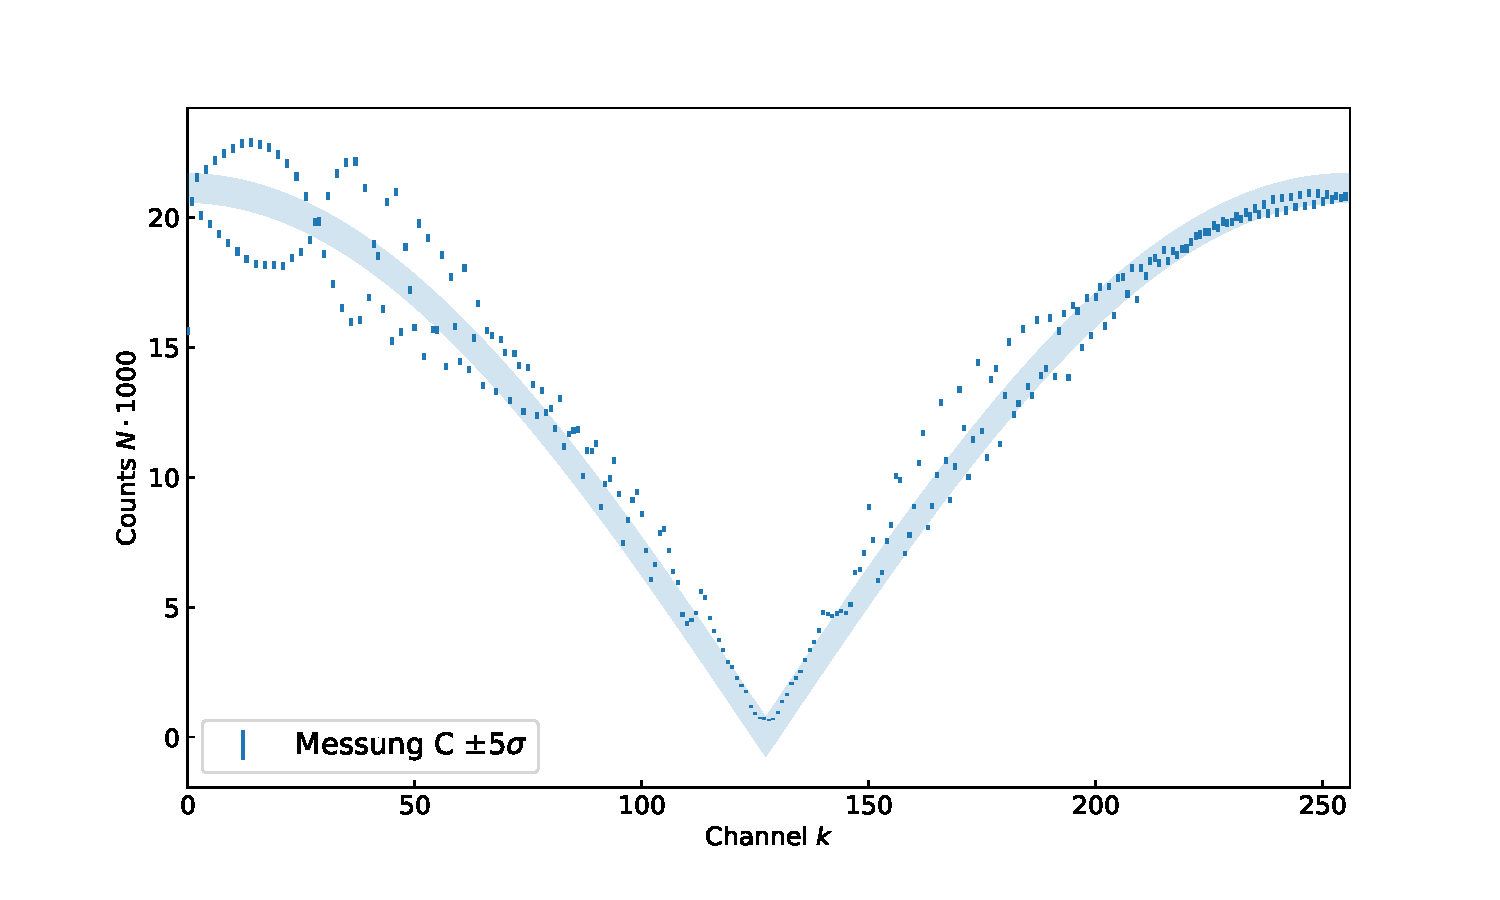
\includegraphics[width=0.7\textwidth]{dat/velocityC.pdf}
	\caption{Kalibrierung für die Messung C. Eingezeichnet sind die ungefilterten Messwerte und die Fitfunktion mit $A = (2,114 \pm 0,011) \cdot 10^4$ und $\Phi=0,7 \pm 0,6$.}
	\label{fig:velocityC}
\end{figure}

Auch in dieser Kalibrierung ist $\Phi = 0,7 \pm 0,6$ sehr nahe an Null.

\subsubsection{Isomerieverschiebung}

Um die Isomerieverschiebung zu erhalten, wird das Spektrum der durch den Absorber transmittierten Strahlung aufgenommen.
Das Signal wird mit einem Diskriminator auf den zu untersuchenden Bereich um $\SI{14,4}{\kilo\electronvolt}$ beschränkt
	und über einen Analog-Digital-Wandler auf den Computer gebracht.
Das gemessene Spektrum ist in Abb. \ref{fig:IsomerieC} zu sehen.

\begin{figure}[ht]
	\centering	
	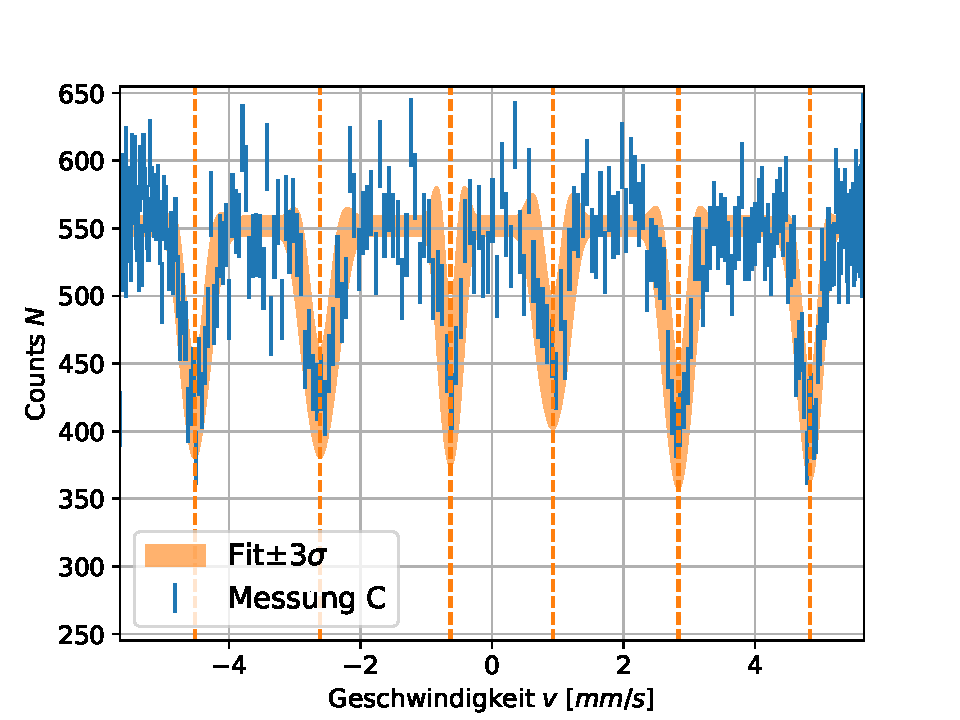
\includegraphics[width=0.8\textwidth]{dat/messungC.pdf}	
	\caption{Isomeriemessungen für Probe C.
		Es ist ein Gaußfit mit sechs Peaks eingezeichnet.
		Die Positionen der Peaks sind der Tab. \ref{isoC} zu entnehmen.
		Aus dem Mittel aller Peaks ergibt sich $v_\test{iso, C} = \input{dat/messungC_iso.txt}$.}
	\label{fig:IsomerieC}
\end{figure}

Für die Aufspaltung durch ein magnetisches Feld ergeben sich sowohl beim Grundzustand, als auch beim angeregten Zustand $2I + 1$ Energieniveaus, welche gleichmäßig um die ungestörte Energie verteilt sind.
Die Isomerieverschiebung kann dann durch Mittelung aller Peakpositionen auf

\begin{equation*}
	v_\text{iso, C} = \frac{1}{6} \sum_{i=1}^6 v_i = \input{dat/messungC_iso.txt}
\end{equation*}

\noindent ermittelt werden.
Damit lässt sich das Material des Absorbers auf $\alpha$-Fe bestimmen, welches laut \ref{TODO:Materialvergleich} eine Isomerieverschiebung
	relativ zu $^{57}$Fe in Pd von \Si{-0.1798 \pm 0.0018}{\milli\meter\per\second} aufweist.

Die entsprechenden Aufspaltungsenergien beider Zustände können in Tab. \ref{tab:isoC} abgelesen werden.
Sie ist definiert als Differenz von Anregungsenergie zu Isomerieverschiebung.

\begin{table}[ht]
	\centering
	\caption{Energieaufspaltungen aller sechs Peaks von Probe C.} 
	\label{tab:isoC}
	\begin{tabular}{c|ccc}
		\toprule
		       &       $v_\text{res}$         &     \Delta v_\text{iso}      &     $\Delta E_\text{iso}$     \\ \midrule
		Peak 1 & \input{dat/messungC_x_5.txt} & \input{dat/messungC_v_5.txt} & \input{dat/messungC_E_5.txt}  \\
		Peak 2 & \input{dat/messungC_x_4.txt} & \input{dat/messungC_v_4.txt} & \input{dat/messungC_E_4.txt}  \\
		Peak 3 & \input{dat/messungC_x_3.txt} & \input{dat/messungC_v_3.txt} & \input{dat/messungC_E_3.txt}  \\
		Peak 4 & \input{dat/messungC_x_2.txt} & \input{dat/messungC_v_2.txt} & \input{dat/messungC_E_2.txt}  \\
		Peak 5 & \input{dat/messungC_x_1.txt} & \input{dat/messungC_v_1.txt} & \input{dat/messungC_E_1.txt}  \\
		Peak 6 & \input{dat/messungC_x_0.txt} & \input{dat/messungC_v_0.txt} & \input{dat/messungC_E_0.txt}  \\ \bottomrule
	\end{tabular}
\end{table} 

\subsubsection{Elektronendichte}

Um die Elektronendichte $\abs{\Psi(0)}^2_\text{A}$ des Absorbers im Kern zu ermitteln, wird Gl. \ref{TODO:formelElektronendichteInAnleitung} nach
\begin{equation}
	\abs{\Psi(0)}^2_\text{A} = \frac{5 v_\text{iso} E_\gamma \varepsilon_0}{S'(Z = 26) c e^2 Z R^2} \frac{1}{\frac{\Delta R}{R}} + \abs{\Psi(0)}^2_\text{Q} = \input{electrondensity_C.txt}
\end{equation}
umgestellt.
Dabei sind $\frac{\Delta R}{R} = TODO:value(dRR)$ aus \ref{TODO:jannikTeilAdRR} bekannt und die Elektronendichte $\abs{\Psi(0)}^2_\text{Q} = \SI{11881,8}{a_0^{-3}}$ von $^57$Fe in Pd gegeben.
Weiter sind $E_\gamma = \SI{14,4}{keV}$ die Quellphotonenenergie, $Z=26$ die Ordnungszahl von Eisen,
    $S'(Z = 26) = 1,33$ der relativistische Korrekturfaktor von Eisen und $R = 1,3 \cdot A^\frac{1}{3} \si{\femto\meter}$ der Kernradius mit $A=57$ für Eisen.

\subsubsection{Magnetische Hyperfeinaufspaltung}

Durch die Hyperfeinstruktur des Kerns sind bei Probe C mehrere diskrete Übergänge möglich.
Der angeregte Zustand mit $I_\text{a} = \frac{3}{2}$ spaltet sich so in die 4 Zustände mit $M\text{a} = -\frac{3}{2}, -\frac{1}{2}, \frac{1}{2}, \frac{3}{2}$ auf,
	während der Grundzustand mit $I_\text{g} = \frac{1}{2}$ die beiden Zustände $M_\text{g} = -\frac{1}{2}, \frac{1}{2}$ annehmen kann.
Durch die Übergangsregeln $\Delta I = 1$ und $\Delta M = \pm 1, 0$ sind gerade die sechs sichtbaren Peaks als Übergänge erlaubt.

\begin{figure}[ht]
	\centering
	\includegraphics[width=0.5\textwidth]{img/transition.svg}
	\caption{}
	\label{fig:transition}
\end{figure}

\noindent Aus Fig. \ref{fig:transition} ist erkennbar, dass 1 die größte und 6 die kleinste Energiedifferenz aufweißt.
Außerdem ist schnell ersichtlich, dass 2 die zweitgrößte und 5 die zweitkleinste Differenz hat.
Damit kann man ihnen diese Peaks im Spektrum zuweisen.
Die Peaks 3 und 4 können noch nicht zugeordnet werden, da sie sich nur um $\Delta E_\text{a} - \Delta E_\text{g}$ unterscheiden.

Mit den Energiedifferenzen von Peak 1 und 2 bzw. 5 und 6 kann nun

\begin{equation}
	v_\text{iso} = - \frac{c}{E_\gamma} \right( \mu_\text{a} \frac{M_\text{a}}{I_\text{a}} - \mu_\text{g} \frac{M_\text{g}}{I_\text{g}} \left) B
\end{equation}

aufgelöst werden.
Dabei sind $v_\text{iso}$ die Resonanzgeschwindigkeit des jeweiligen Peaks, $E_\gamma = \SI{14,4}{\kilo\electronvolt}$ die Photonenenergie der Quelle, $B$ das Magnetfeld im Kern und $\mu_\text{a,g}$ das magnetische Moment sowie $I,M$ die Quantenzahlen des angeregten oder des Grundzustandes.
Das magnetische Moment des Grundzustandes ist bekannt und beträgt $\mu_\text{g} = \SI{0,09044 \pm 0,00007}{\mu_N}$.
Setzt man die Werte von einem Paar ein und löst das Gleichungssystem, so ergeben sich $B =  - \frac{v_1 + 3 v_2}{c} \frac{E_\gamma}{2 \mu_\text{g}}$
	und $\mu_\text{a} = 3 \mu_\text{g} \frac{v_1+v_2}{v_1 + 3 v_2}$.
Für 1 und 2 folgt $B_{1,2} = \input{dat/B_Feld_12.txt}$ und $\mu_\text{a, 1,2} = \input{dat/mu_A_12.txt}$.
Für 5 und 6 folgt $B_{5,6} = \input{dat/B_Feld_56.txt}$ und $\mu_\text{a, 5,6} = \input{dat/mu_A_56.txt}$.

Aus der Form der Messung Fig. \ref{fig:IsomerieC} kann abgeleitet werden, dass es sich um unmagnetisiertes $\alpha$-Fe handelt.
Das ist daran zu erkennen, dass sechs Peaks gemessen worden sind, welche zu höheren Geschwindigkeiten hin an Amplitude gewinnen.
Allerdings ist nicht das erwartete Verhältnis von 1:2:3 gemessen worden.

%%-----------------------------------------------------------%%

% TODO:{Schnell alle Materialien auf einen Blick. Kann rauskopiert und irgendwohin verschoben werden. ggf. noch nen kleinen Text.}
\begin{figure}[ht]
	\centering
	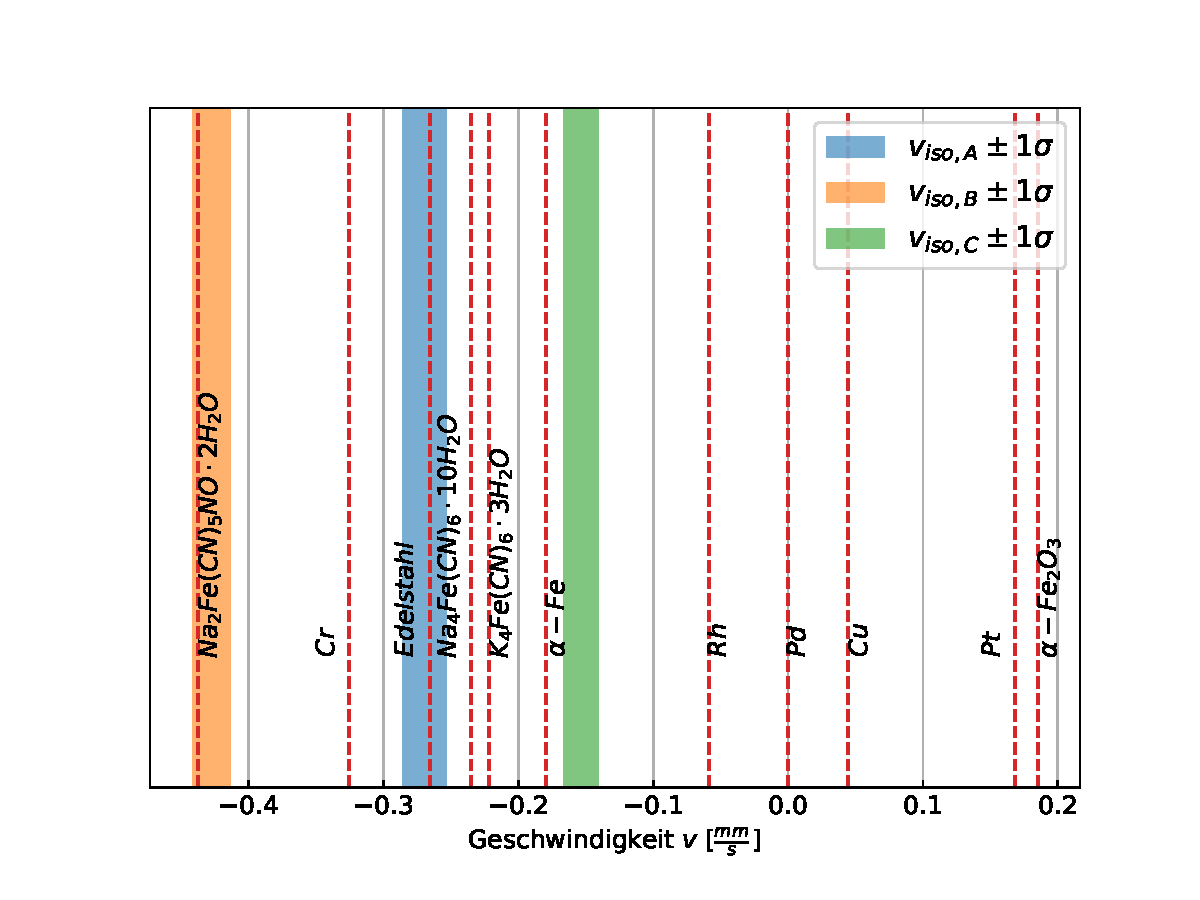
\includegraphics[width=0.7\textwidth]{dat/isoVgl.pdf}
	\caption{Schematische Übergänge in Probe C. }
	\label{fig:isoVgl}
\end{figure}

\begin{table}[ht]
	\centering
	\caption{Absorber und ihre Isomerieverschiebungen.} 
	\label{tab:isoVgl}
	\begin{tabular}{c|ccc}
		\toprule
		  &   $v_\text{iso}$ gemessen    &            $v_\text{iso}$ gegeben             &           Materialname            \\ \midrule
		A & \input{dat/messungA_iso.txt} & \SI{-0.2658+-0.0032}{\milli\meter\per\second} &             Edelstahl             \\
		B & \input{dat/messungB_iso.txt} & \SI{-0.4374+-0.0018}{\milli\meter\per\second} & N$_2$Fe(CN)$_5$NO $\cdot$ 2H$_2$O \\
		C & \input{dat/messungC_iso.txt} & \SI{-0.1798+-0.0018}{\milli\meter\per\second} &             $\alpha$-Fe              \\ \bottomrule
	\end{tabular}
\end{table}

 